\documentclass{beamer}

\usepackage{framed}
\usepackage{graphicx}

\usepackage{amsmath}

\begin{document}
%======================================= %


\begin{frame}
	\begin{figure}
\centering
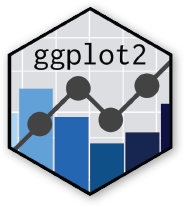
\includegraphics[width=0.45\linewidth]{ggplot2-official-hexbin-logo}
\end{figure}
\large
\[\mbox{Coding Grace - ggplot2 Workshop 2016}\]



\end{frame}


%============================================== %
\begin{frame}
	\Large
	\noindent\textbf{About ggplot2}
	\bigskip
	\begin{itemize}
\item The ggplot2 package, created by Hadley Wickham, offers a powerful graphics language for creating elegant and complex plots. Its popularity in the R community has exploded in recent years. 
\item Originally based on Leland Wilkinson's The Grammar of Graphics, ggplot2 allows you to create graphs that represent both univariate and multivariate numerical and categorical data in a straightforward manner.
%\item  Grouping can be represented by color, symbol, size, and transparency.
	\end{itemize}

\end{frame}
%======================================= %

%========================================== %
\begin{frame}
	\Large
	\noindent\textbf{Benefits of ggplot2}
	
	\begin{enumerate}
		\item ggplot is easy to learn [\textit{1}]
		\item ggplot is fun
		\item ggplot is powerful [\textit{2}]
	\end{enumerate}
	
	\begin{framed}
		\textit{[1] Lots of learning resources, mainly intended for the R environment, that can applied to Python also.}\\
		\bigskip
		\textit{[2] Less code required to compute high-level publication quality plot}
	\end{framed}
	(source: www.yhat.com)
\end{frame}	
%======================================== %
\begin{frame}
	\begin{figure}
		\centering
		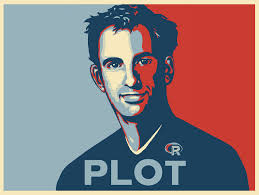
\includegraphics[width=0.95\linewidth]{HW}
	\end{figure}
	Hadley Wickham (Chief Data Scientist, RStudio)
\end{frame}
%======================================== %	
\begin{frame}
	\begin{figure}
\centering
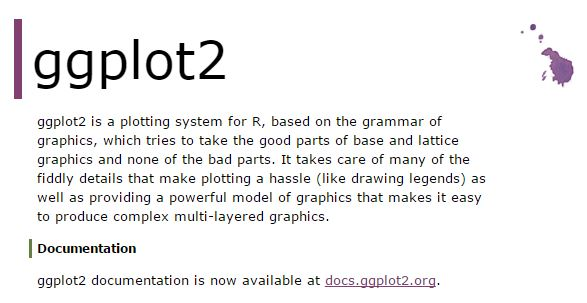
\includegraphics[width=1.15\linewidth]{ggplot2-website}
\end{figure}
website: www.had.co.nz

\end{frame}

%============================================= %

\begin{frame}
\begin{figure}
\centering
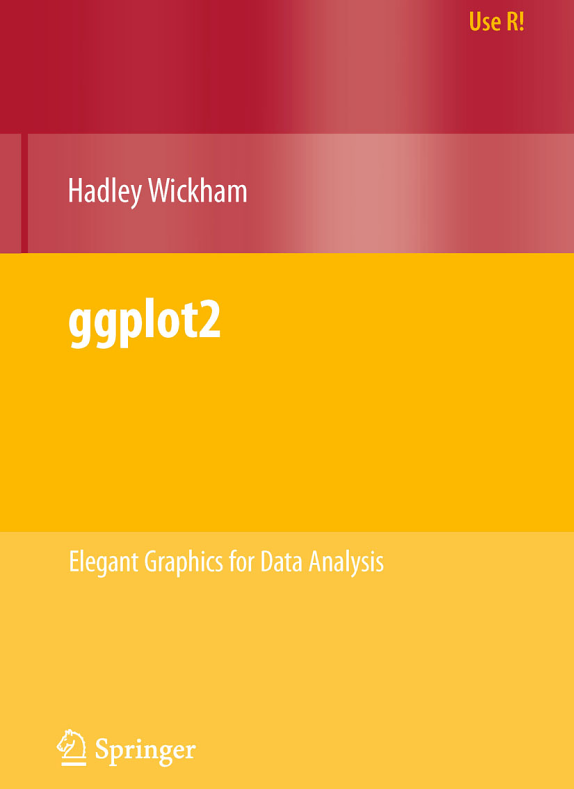
\includegraphics[width=0.55\linewidth]{ggplot2-bookcover}
\end{figure}
ggplot2: Elegant Graphics for Data Analysis
\end{frame}

%============================================= %
\begin{frame}
	\frametitle{Prof. Dianne Cook (Monash University)}
\begin{figure}
\centering
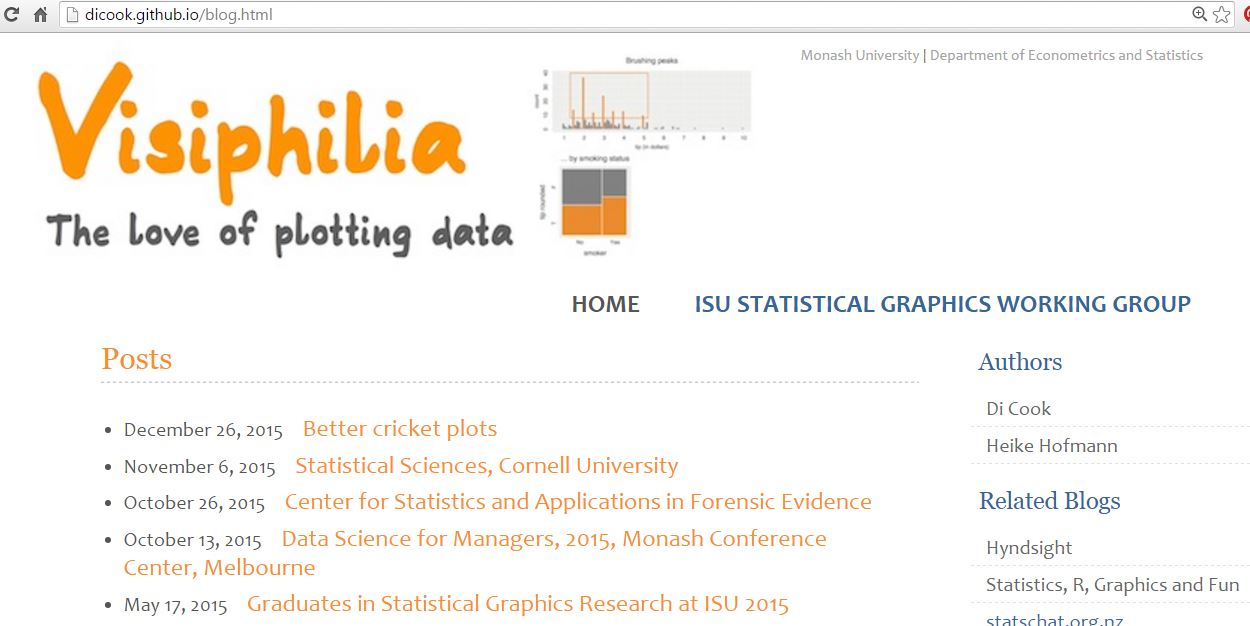
\includegraphics[width=1.1\linewidth]{visiphilia}
\end{figure}
\end{frame}



%===================================== %
\begin{frame}[fragile]
\textbf{1. Installing ggplot2}
\begin{framed}
\begin{verbatim}
install.packages("ggplot2")

library(ggplot2)
\end{verbatim}
\end{framed}
N.B. Not installed automatically with \texttt{R}.
\end{frame}

%================================================================================== %
\begin{frame}[fragile]
	\frametitle{Data}
	\Large
	\vspace{-1.4cm}\begin{figure}
\centering
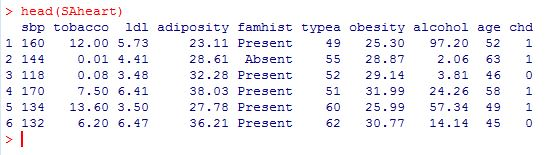
\includegraphics[width=0.9\linewidth]{SAhearts-dataframe}

\end{figure}

	\begin{itemize}

		\item If you're planning on using ggplot2, it's best to keep your data in \texttt{data.frame} . 
		\item Think of a \texttt{data.frame} as a tabular data object. 
%		\item For example, let's look at the diamonds dataset which ships with ggplot.
	\end{itemize}
\end{frame}

%============================================= %
\begin{frame}[fragile]
	\frametitle{Anscombe Quartet}
	\Large
\begin{itemize}
	\item  In 1973, the statistician Francis Anscombe demonstrated the importance of graphing data.
	\item  The Anscombe's Quartet shows how four sets of data with identical simple summary statistics can vary considerably when graphed.
\end{itemize}

\end{frame}
%============================================= %
\begin{frame}[fragile]

	\begin{figure}
		\centering
		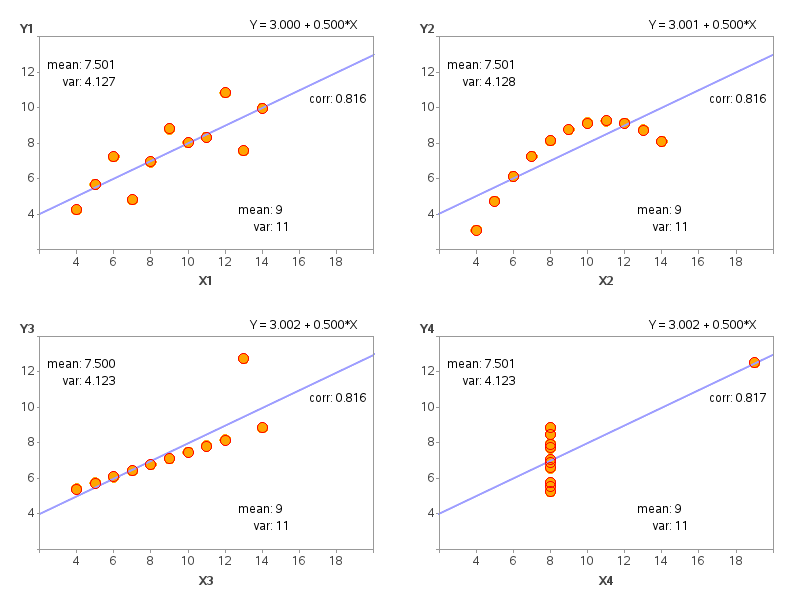
\includegraphics[width=1.0\linewidth]{anscombe4}
	\end{figure}
(Source: Wikipedia)
\end{frame}
%=======================================================%
\begin{frame}[fragile]
\Large
Try this out!
\begin{framed}	\begin{verbatim}
ggplot(aes(x=x1, y=y1), data=anscombe2)
 + facet_wrap(group,scales=fixed) 
 + geom_point()
 + stat_smooth(method="lm")

	\end{verbatim}\end{framed}
\end{frame}
%============================================= %

\begin{frame}
	\frametitle{ggplot - Inbuilt Data Sets}
	\Large

Data sets included in ggplot2 and used in examples\smallskip
	\begin{description}


\item[diamonds]
Prices of 50,000 round cut diamonds


\item[faithfuld]
2d density estimate of Old Faithful data


\item[midwest]
Midwest demographics.

\item[mpg]
Fuel economy data from 1999 and 2008 for 38 popular models of car

\item[msleep]
An updated and expanded version of the mammals sleep dataset.




\item[txhousing]
Housing sales in Texas.
	\end{description}

\end{frame}

%===================================== %
\begin{frame}[fragile]
\Large
\begin{itemize}
\item The main command is \texttt{ggplot()}.
\item The name comes from "\textbf{grammar of graphics}", a book by Leland Wilkinson
\item A very ``high-level" approach to data visualization.
\end{itemize}
{
	\large
\begin{framed}
\begin{quote}
	A grammar of graphics is a tool that enables us to concisely describe the components
	of a graphic. Such a grammar allows us to move beyond named graphics (e.g., the “scatterplot”)
	and gain insight into the deep structure that underlies statistical graphics.
\end{quote}
\end{framed}
}
\end{frame}

\begin{frame}

\begin{figure}
\centering
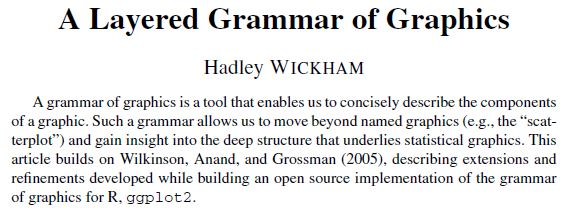
\includegraphics[width=1.1\linewidth]{HWpaper}
\end{figure}
\begin{framed}
Hadley Wickham.\\
\textbf{A layered grammar of graphics.}\\
\textit{Journal of Computational and Graphical Statistics, \\ vol. 19, no. 1, pp. 3–28, 2010.}
\end{framed}

\end{frame}

\section{How it works}
\begin{frame}[fragile]
	\Large
	\frametitle{Basic Premise}
\vspace{-0.7cm}
	\begin{itemize}
		\item Making plots is a very repetive: draw this line, add these colored points, then add these, etc. 
		\item Instead of re-using the same code over and over, \texttt{ggplot} implements them using a high-level but very expressive API.
		\item The result is less time spent creating your charts, and more time interpreting what they mean.
	\end{itemize}
\indent \textit{(From ggplot documentation)}	
\end{frame}

%================================================================================== %
\begin{frame}[fragile]
	\Large
\frametitle{Basic Premise}
\vspace{-0.7cm}
	\begin{itemize}
		\item \texttt{ggplot} is not a good fit for people trying to make highly customized data visualizations. 
		\item \textit{(Compare this to high level ``Bokeh" plots)}
		\item While you can make some very intricate, great looking plots, \texttt{ggplot} sacrifices highly customization in favour of general doing "what you'd expect".
	\end{itemize}
\textit{(From ggplot documentation)}	
\end{frame}

%===================================== %
\begin{frame}[fragile]
	\begin{figure}
		\centering
		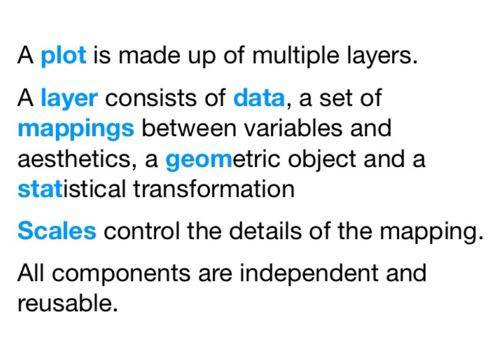
\includegraphics[width=1.1\linewidth]{ggplot2-info}
	\end{figure}
	(Source: Hadley Wickham)
\end{frame}
%================================================================================== %

\section{Layers}
\begin{frame}[fragile]
	\frametitle{Layers}
	\Large
	\noindent \textbf{Layers}
	\begin{itemize}
		\item \textbf{ggplot} lets you combine or add different types of visualization components (or layers) together. 
		%\item I think this is easiest to understand with an example.
		\item The command \texttt{ggplot()} does not actually create any plot, rather it prepares a ``blank canvas" for further plotting .
		\item (We will introduce \textit{geoms} shortly.)
	\end{itemize}
	
\end{frame}

%================================================================================== %
\begin{frame}[fragile]
	\textbf{	Start with a blank canvas.}
	\begin{framed}
		\begin{verbatim}
		# meat data set (meat2.csv)
		
		p <- ggplot(aes(x=date, y= beef), data=meat2)
		p
		\end{verbatim}
	\end{framed}
	\begin{figure}
		\centering
		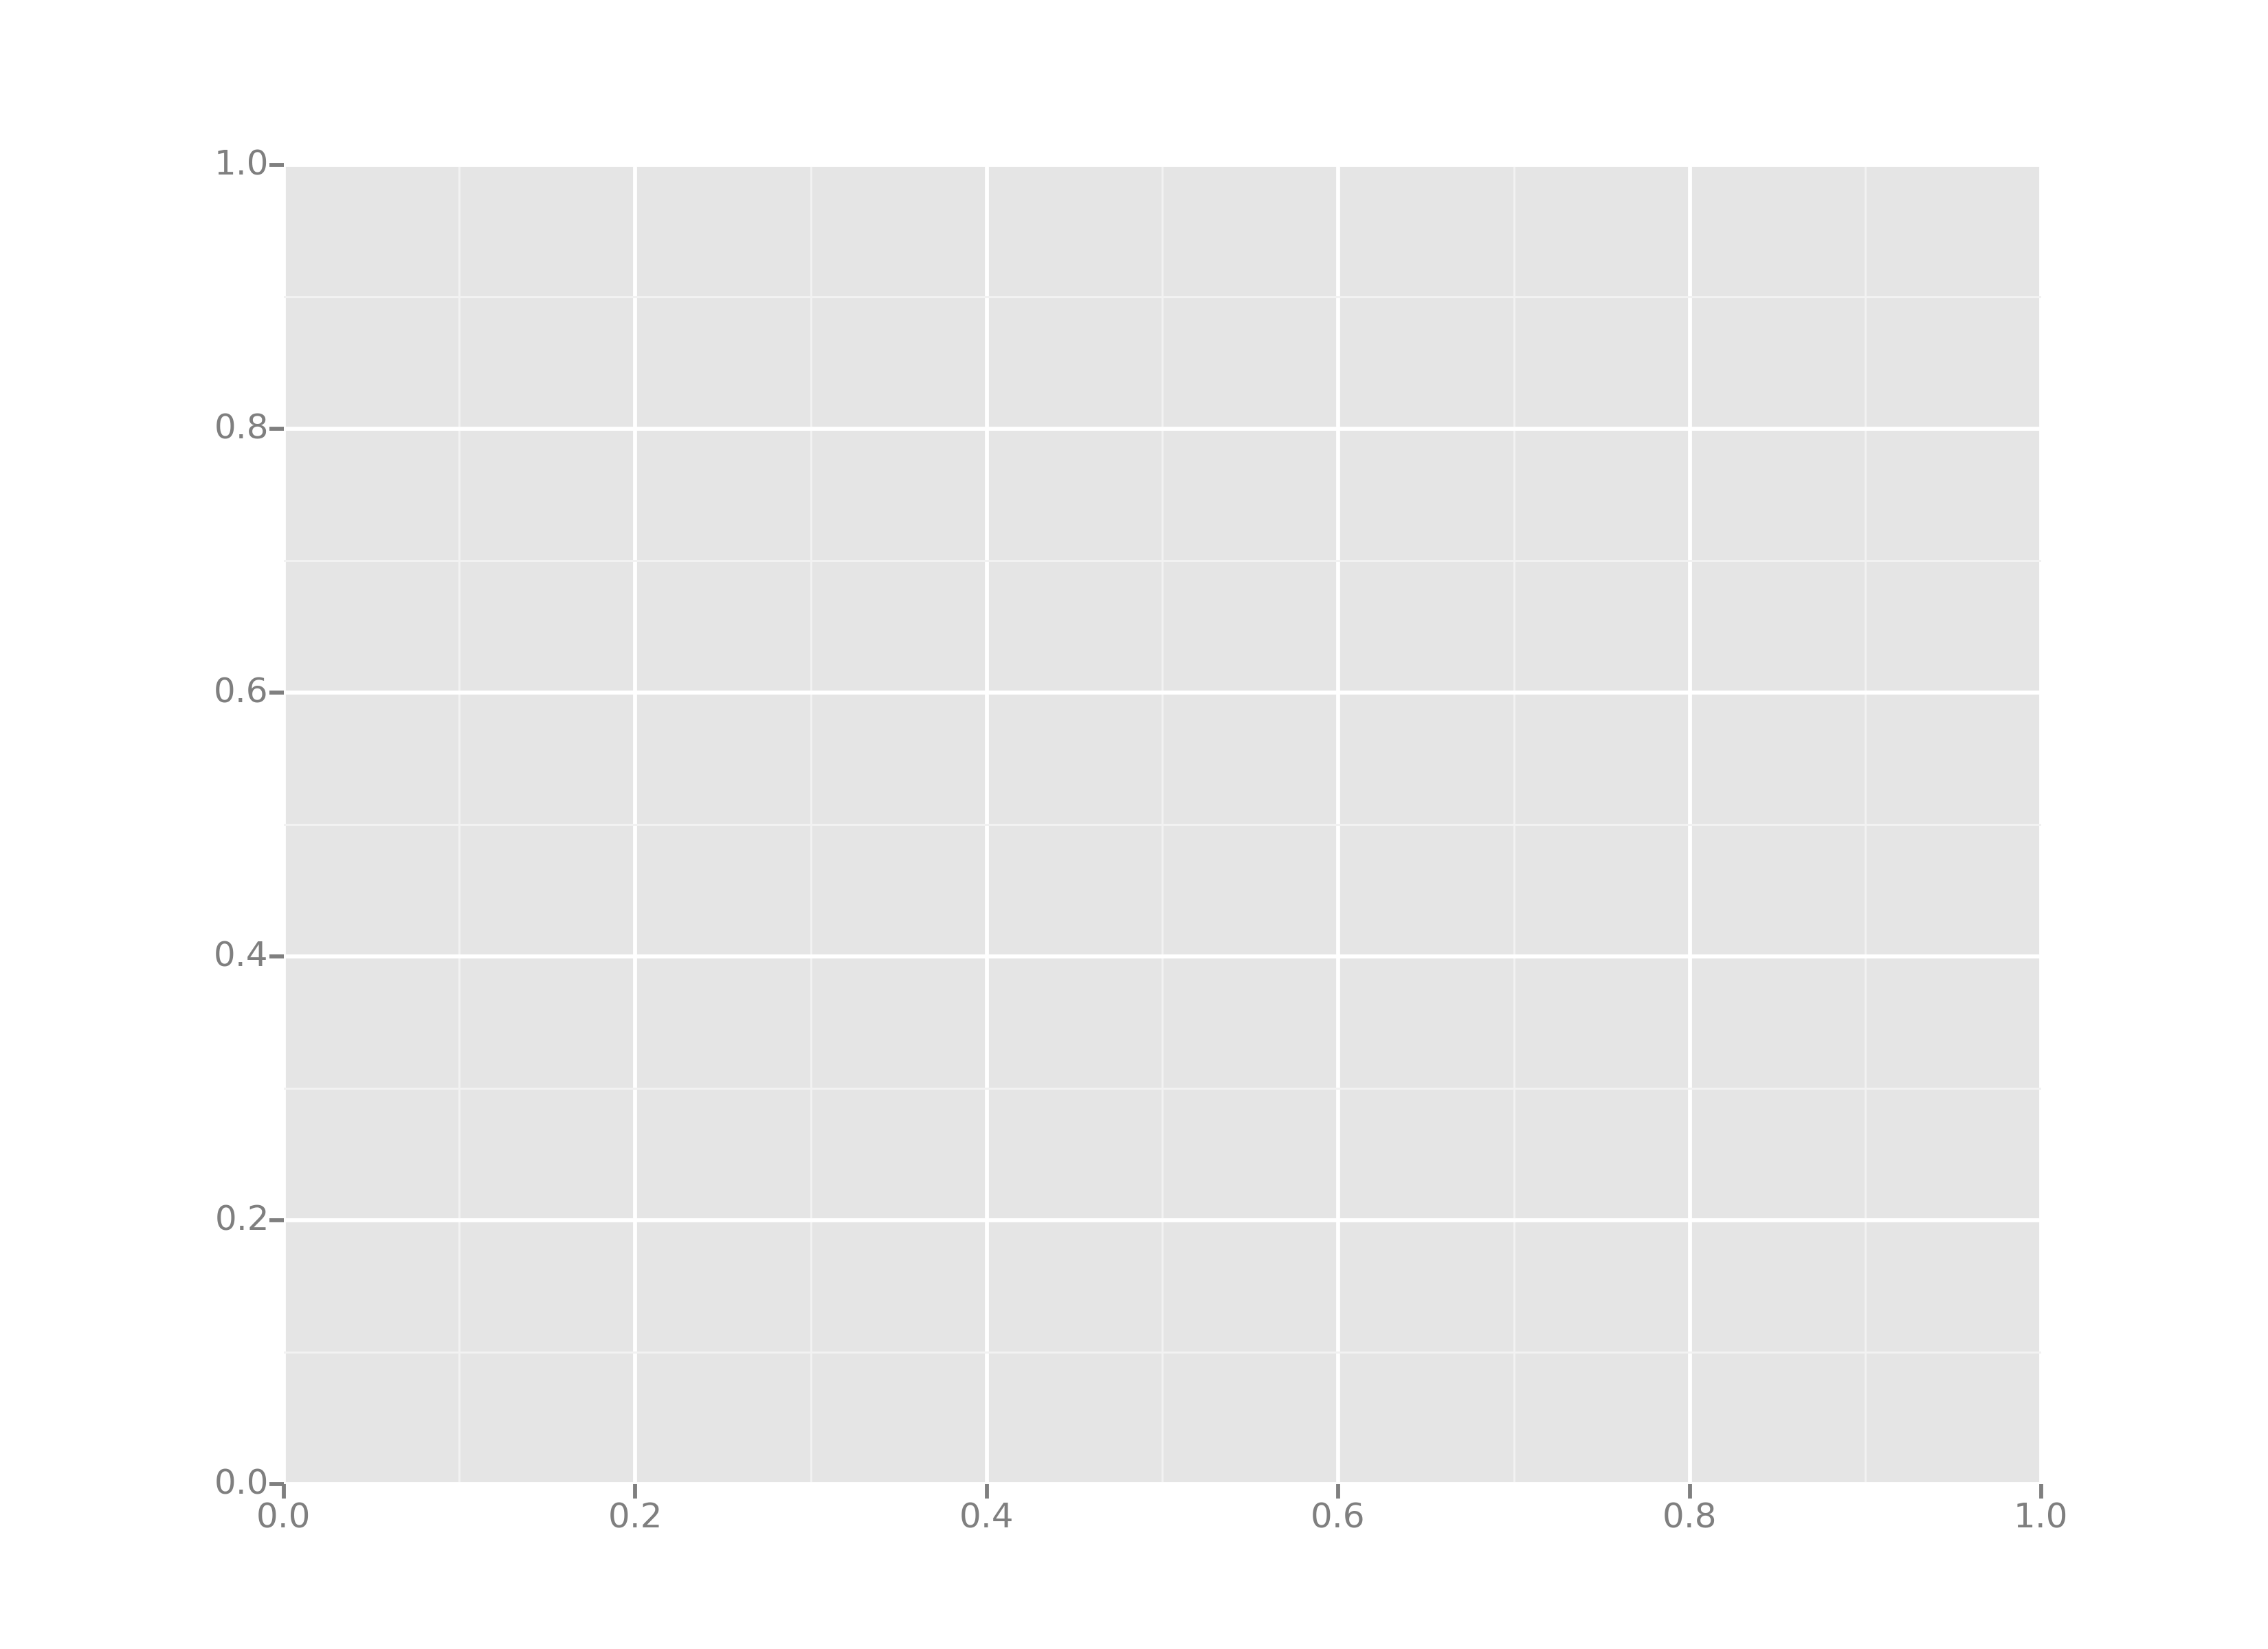
\includegraphics[width=0.5\linewidth]{Layers1}
	\end{figure}
	
\end{frame}
\begin{frame}[fragile]
	\vspace{-0.7cm}
\textbf{Lets try these exercises out with different data sets (both inbuilt)}
	\begin{framed}
		\begin{verbatim}
	p1 <- ggplot(aes(x=wt, y=mpg), 
	       data=mtcars)
	       
	p2 <- ggplot(aes(x=depth, y=carat), 
	               data=diamonds)
		\end{verbatim}
	\end{framed}

	
\end{frame}
%================================================================================== %
\begin{frame}[fragile]
\textbf{	Add some points.}
	\begin{framed}
		\begin{verbatim}
		p + geom_point()

		\end{verbatim}
	\end{framed}
	\begin{figure}
		\centering
		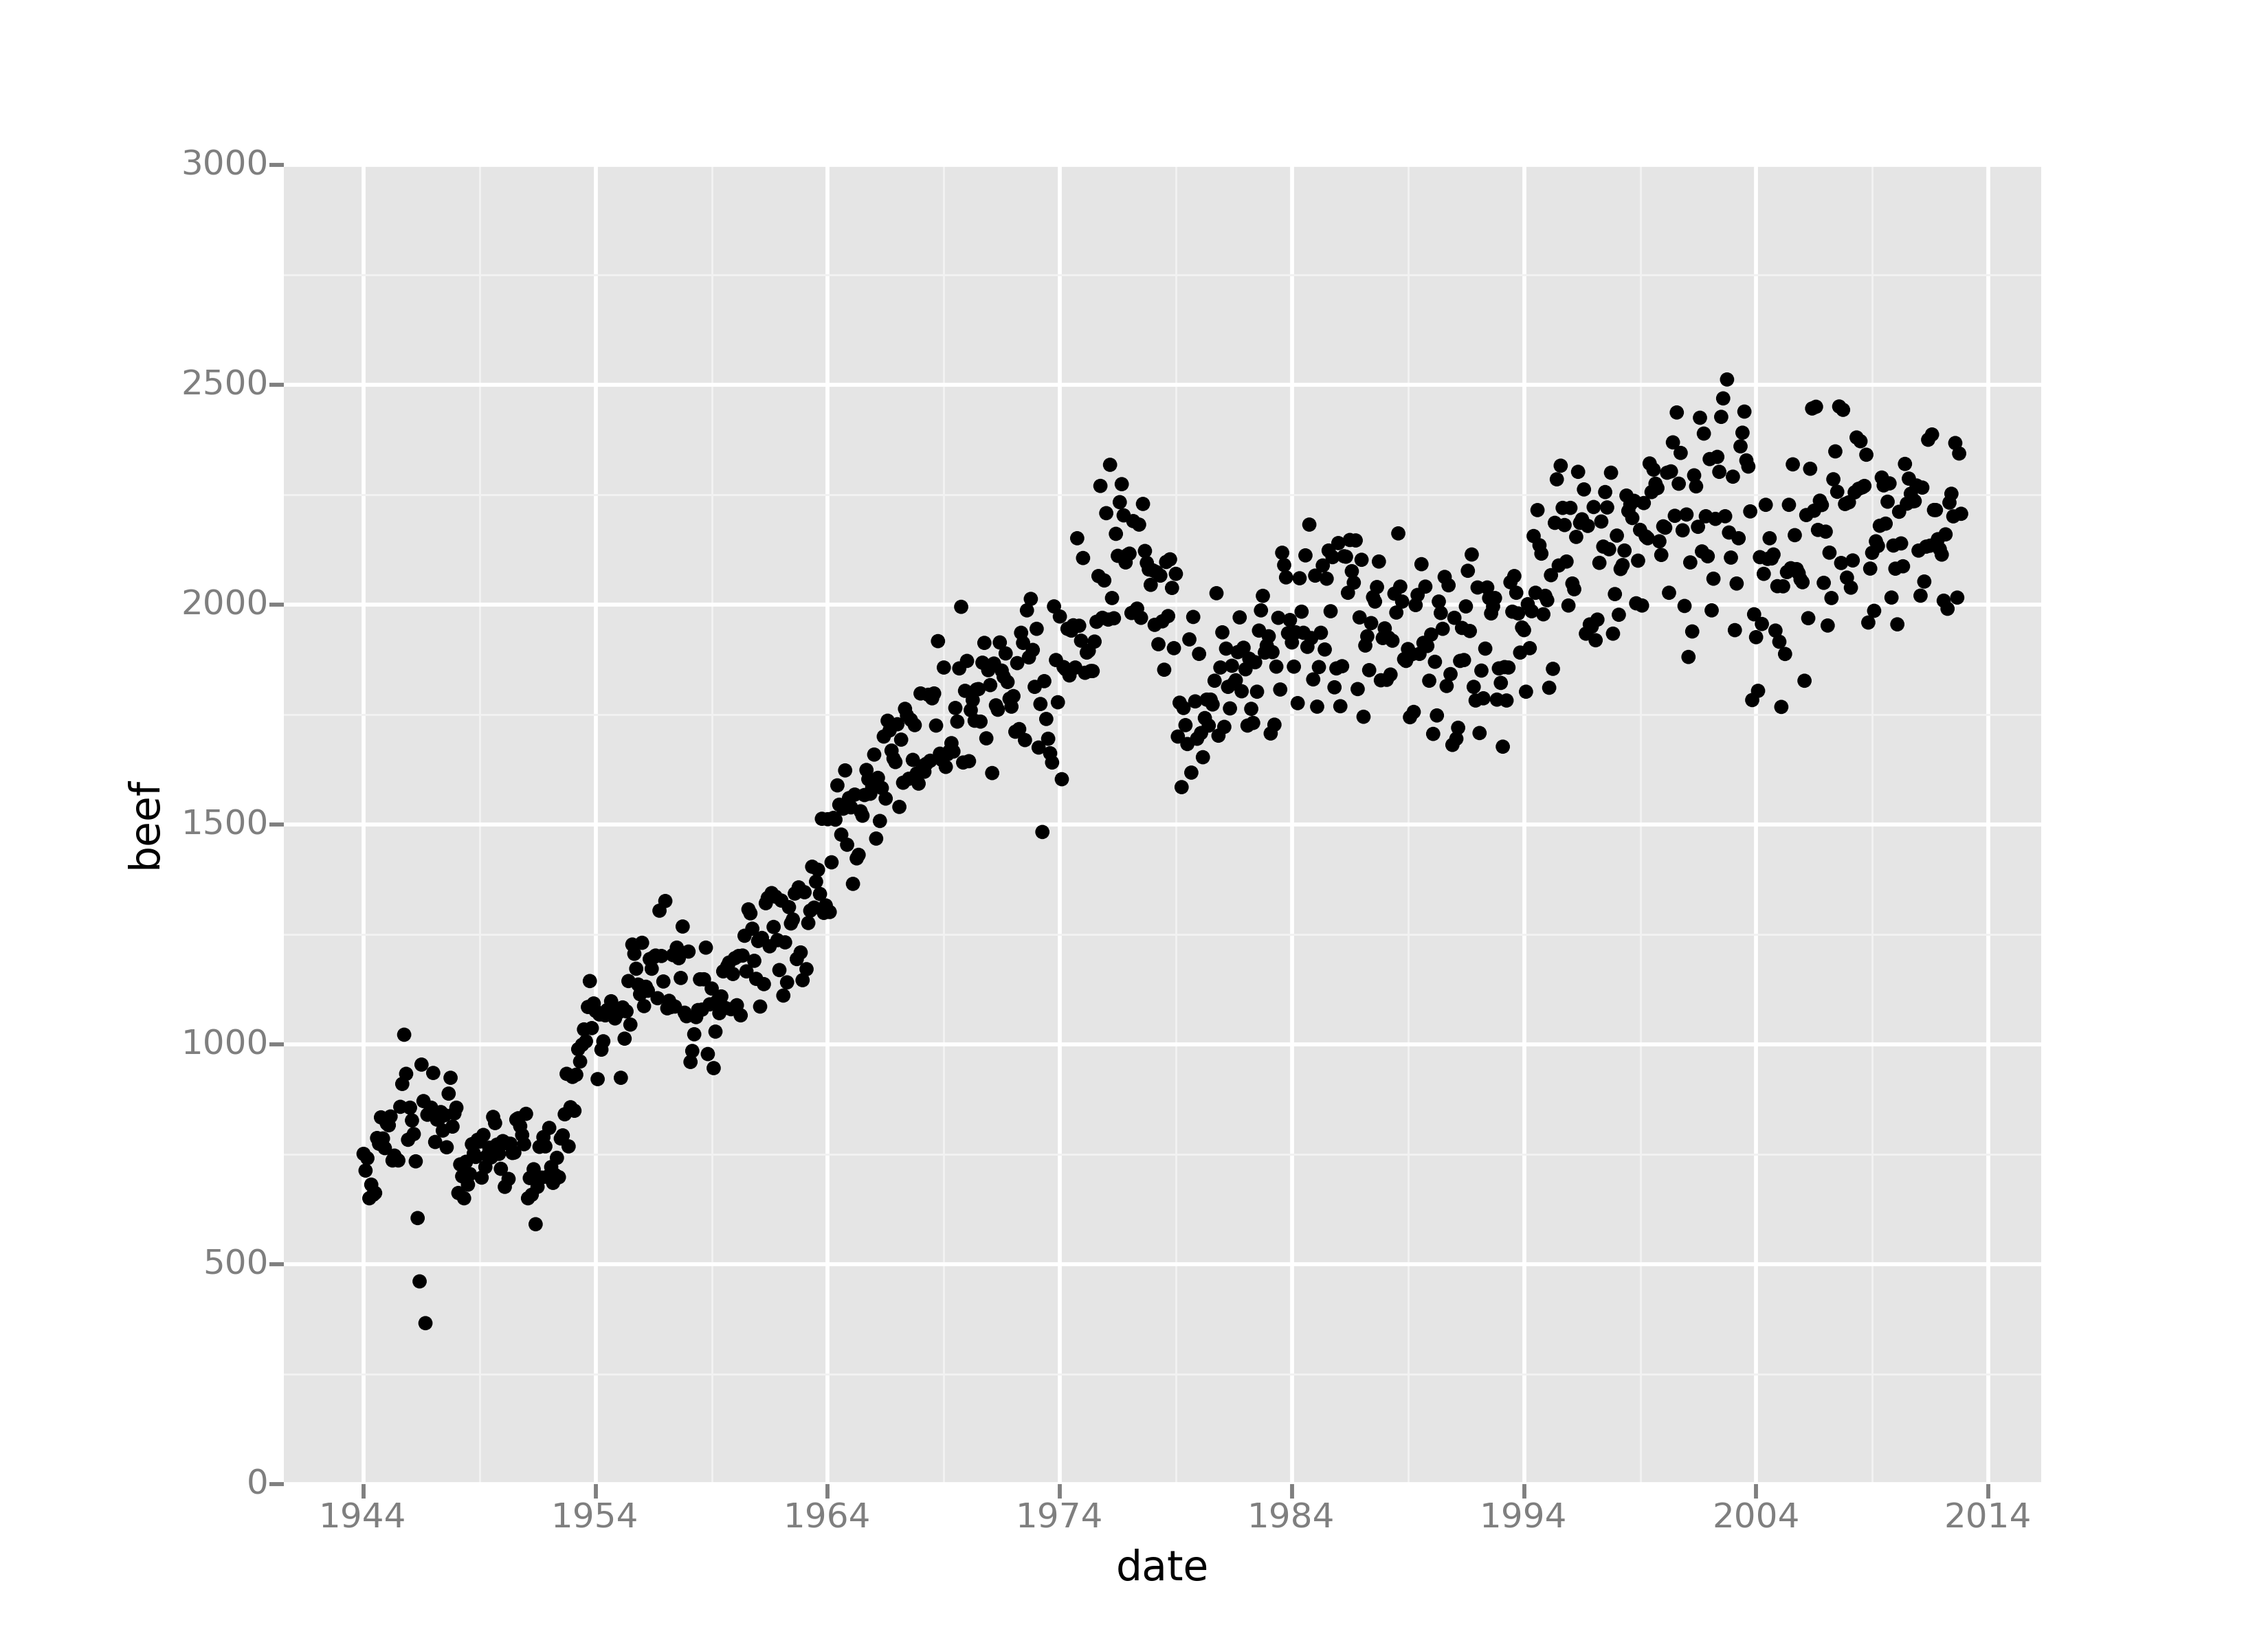
\includegraphics[width=0.7\linewidth]{Layers2}
	\end{figure}
	
	
\end{frame}
\begin{frame}[fragile]
%	\frametitle{ ggplot - Layers}
\textbf{	Add a line.}
	\begin{framed}
		\begin{verbatim}
		p + geom_point() + geom_line()
		\end{verbatim}
	\end{framed}
	\begin{figure}
		\centering
		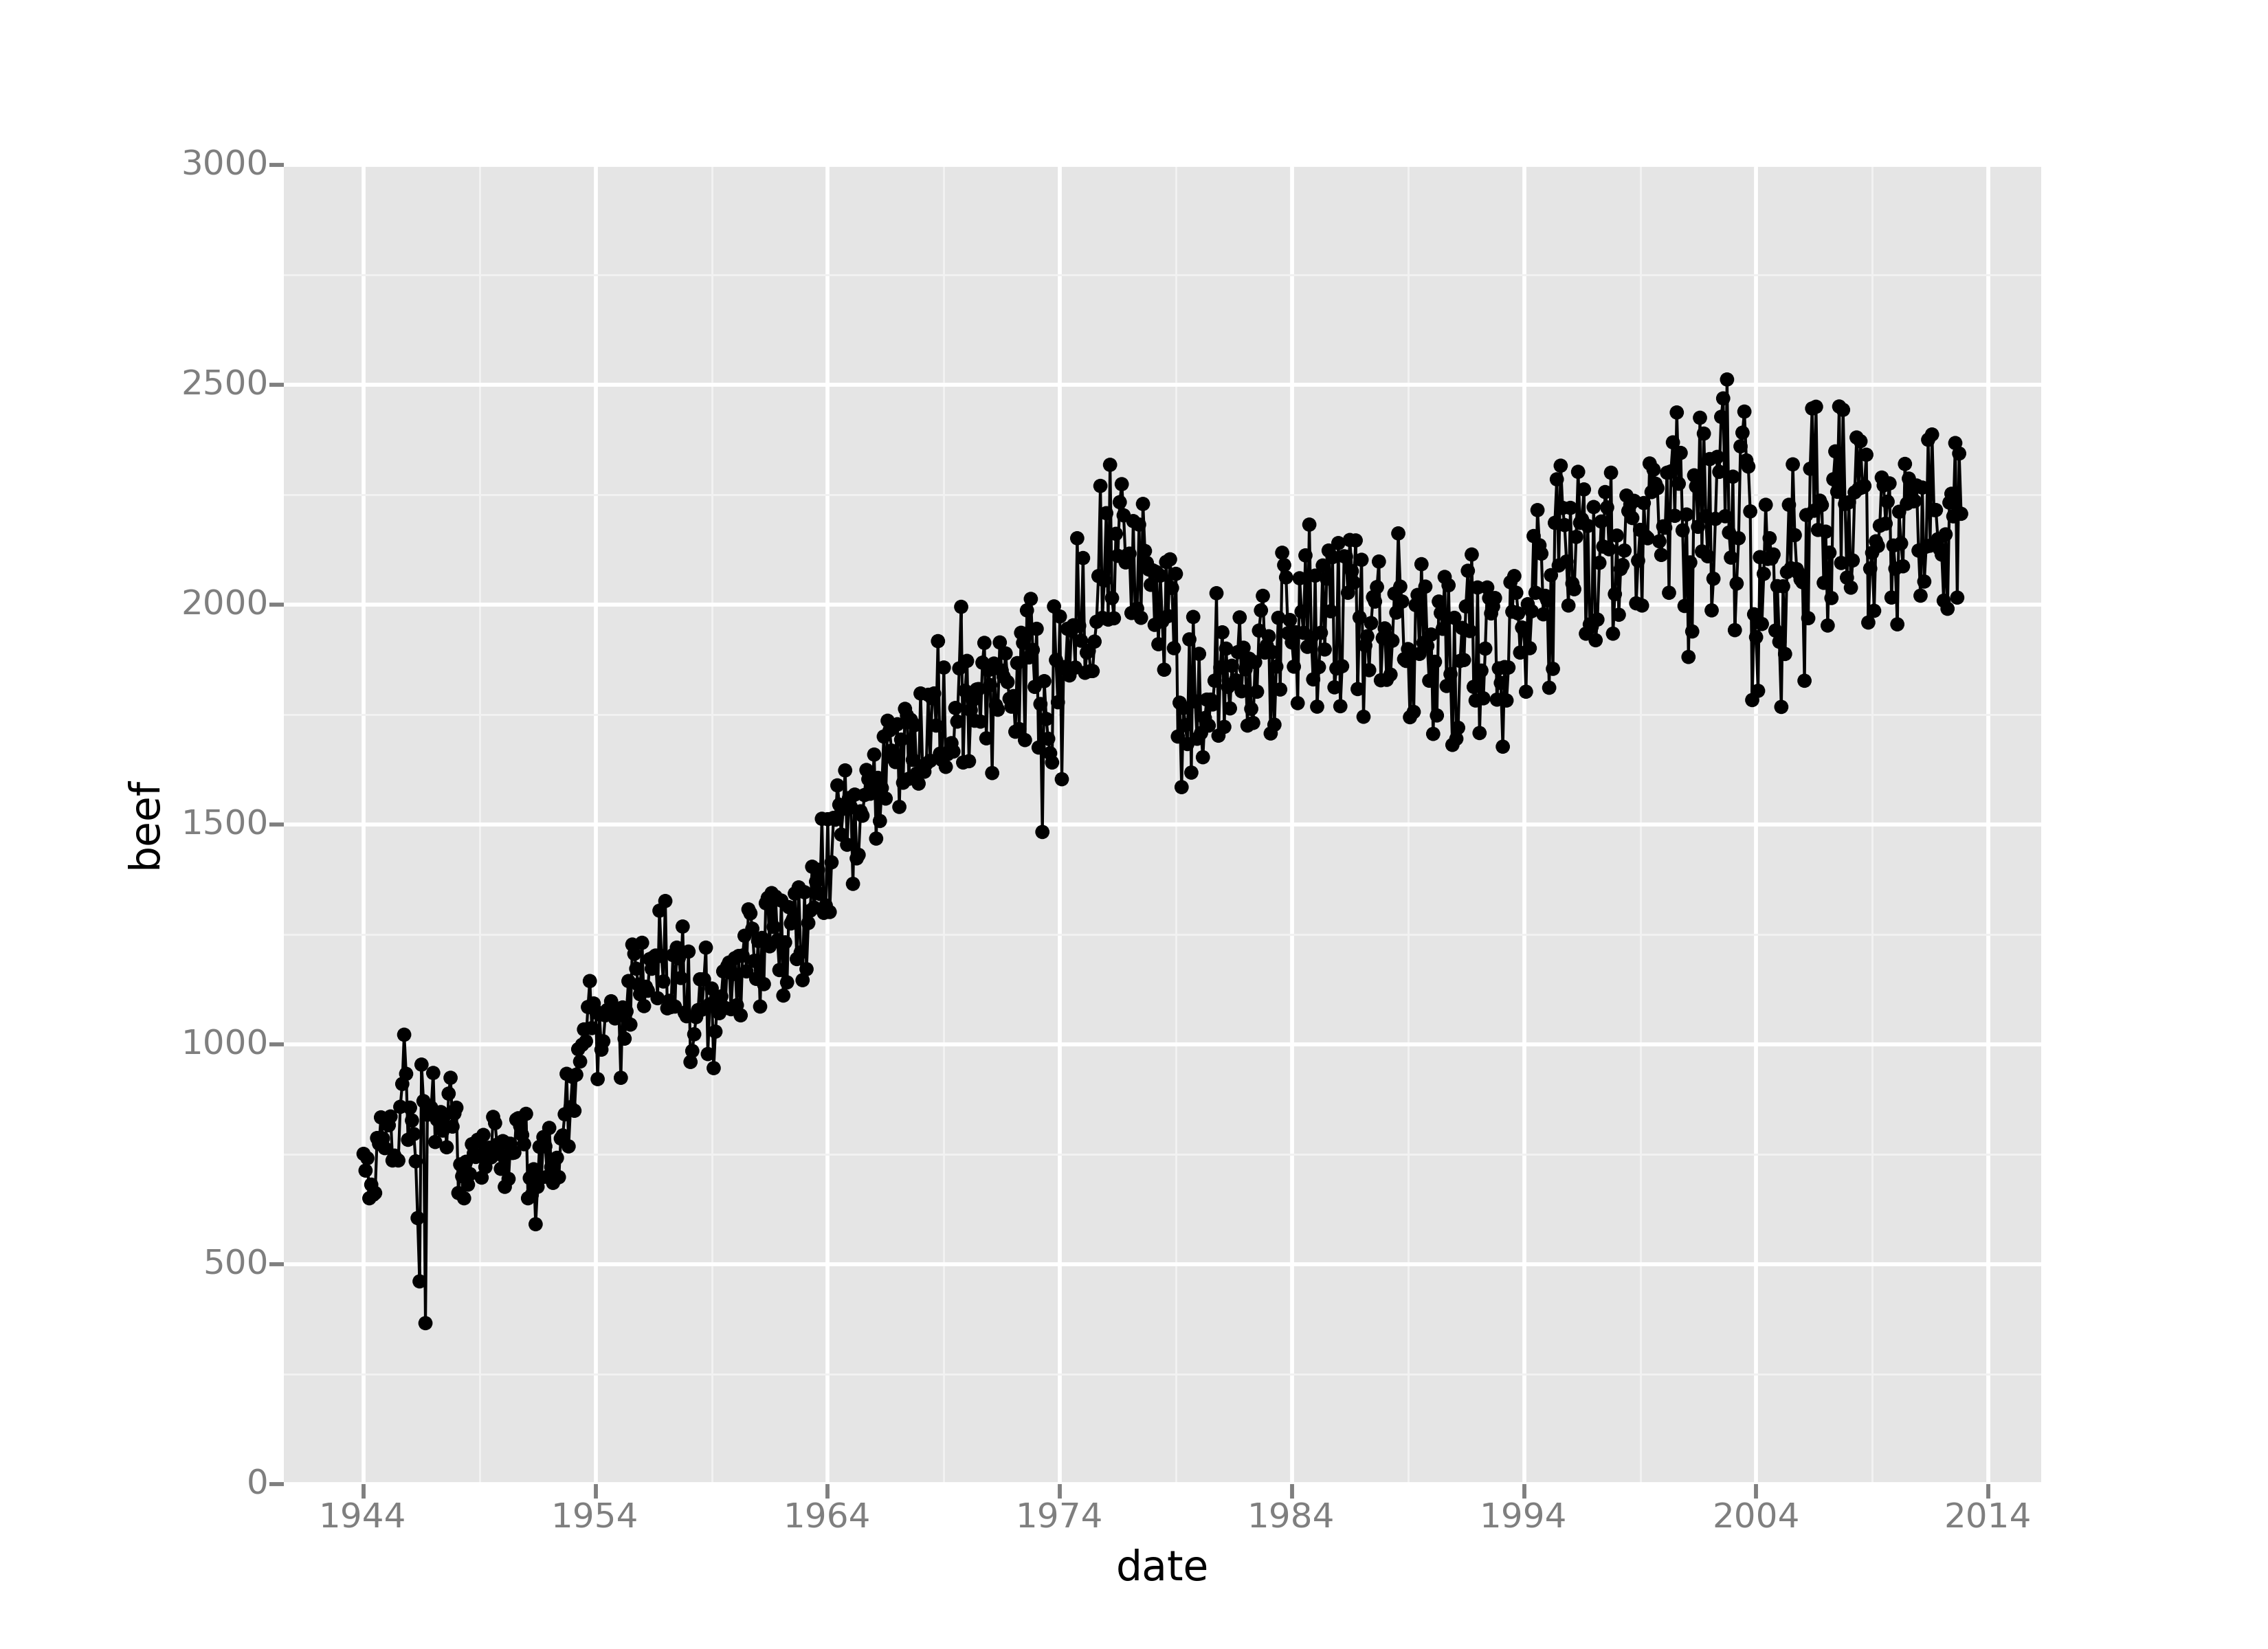
\includegraphics[width=0.7\linewidth]{Layers3}
	\end{figure}
	
\end{frame}

%================================================================================== %
\begin{frame}[fragile]
%	\frametitle{ ggplot - Layers}
\textbf{	Add a trendline.}
	\begin{framed}
		\begin{verbatim}
		p + geom_point() + geom_line() +
		stat_smooth(color="blue")
		\end{verbatim}
	\end{framed}
	\begin{figure}
		\centering
		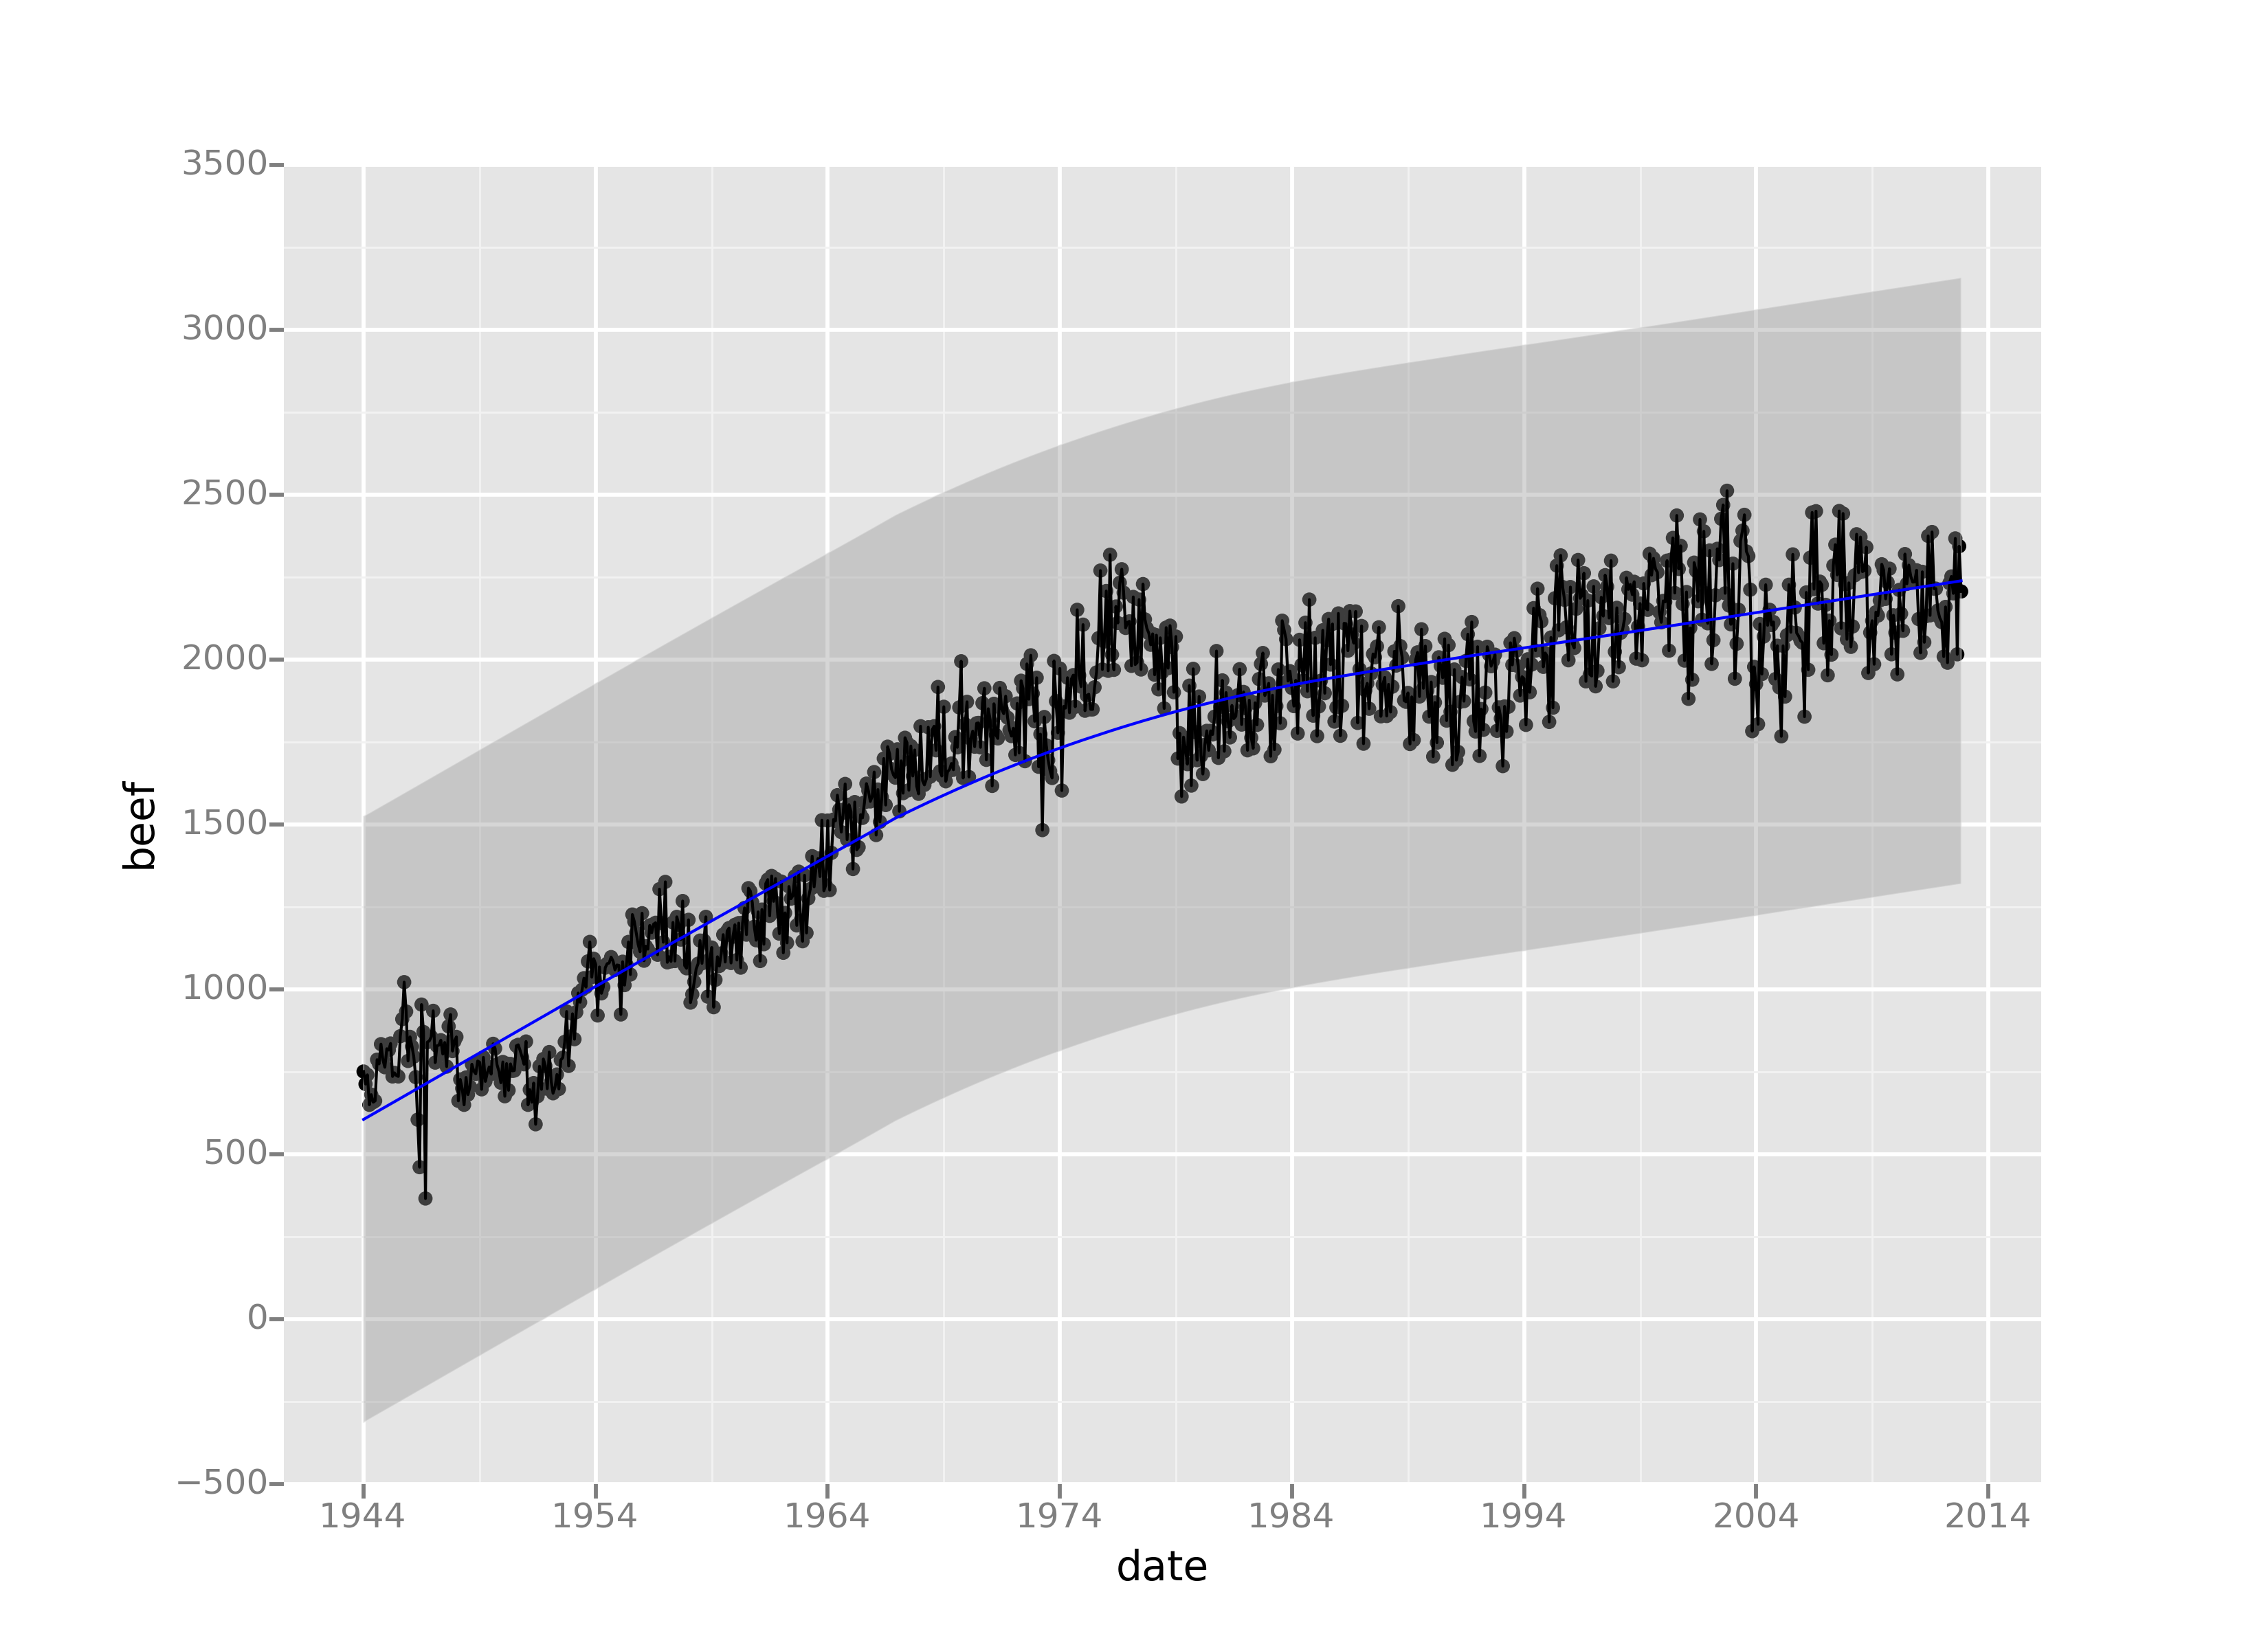
\includegraphics[width=0.7\linewidth]{layers4}
	\end{figure}
\end{frame}

\begin{frame}[fragile]
\frametitle{qplot}
\Large
\vspace{-2cm}
More!
\begin{framed}
\begin{verbatim}
p + ggtitle("Plot Title") 
  + xlab(" X Axis Label") 
  + ylab(" Y Axis Label")

\end{verbatim}
\end{framed}
\end{frame}

\begin{frame}
	\frametitle{Aesthetics}
	\Large
	\noindent \textbf{Rule of Thumb}
	\begin{itemize}
		\item The \texttt{aes} argument is for aesthetics
		\item Essentially it identifies which variables are being used, and in what order.
		\item The first two variables are the ``X" and ``Y" variable.
		\item Anymore variables after that are typically grouping variables (categorical).
	\end{itemize}
\end{frame}
%================================================================================== %
\begin{frame}[fragile]
	\frametitle{Aesthetics}
	\Large
%The first aesthetic variable is for \texttt{color}. This can be used to depict subcategories in the data.
	\begin{framed}
		\begin{verbatim}
ggplot(diamonds, aes(x=carat, 
  y=price, color=cut))+
  geom_point()
	\end{verbatim}
\end{framed}

\end{frame}
%================================================================================== %
\begin{frame}
	
	\begin{figure}
\centering
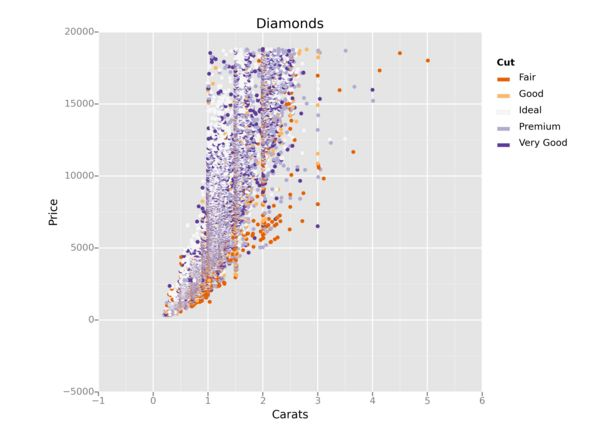
\includegraphics[width=1.1\linewidth]{aesthetic2}
\end{figure}

\end{frame}
%================================================================================== %
%================================================================================== %

%=========================== %
\section{Geoms}
\begin{frame}
	\frametitle{geoms}
	\Large
	Geometric objects (geoms) are the visual representations of (subsets of) observations.\smallskip
	\begin{itemize}
		\item \textbf{Univariate} - single numeric variable
		\item \textbf{Bivariate} - two numeric variable
		\item \textbf{Multivariate} - Multiple variables
	\end{itemize}
\end{frame}
%================================ %
\begin{frame}
	\frametitle{geoms for ggplot}
	\Large
	Here are some of the geoms currently available. \\
	
	\bigskip
	\begin{tabular}{|l|l|l	|}
		\hline
		geom\_abline	&	geom\_histogram	&	geom\_pointrange	\\ \hline
		geom\_area	&	geom\_hline	&	geom\_rect	\\ \hline
		geom\_bar	&	geom\_jitter	&	geom\_smooth	\\ \hline
		geom\_blank	&	geom\_line	&	geom\_step	\\ \hline
		geom\_boxplot	&	geom\_linerange	&	geom\_text	\\ \hline
		geom\_density	&	geom\_path	&	geom\_tile	\\ \hline
		geom\_dotplot	&	geom\_point	&	geom\_vline	\\ \hline
		
		
	\end{tabular} 
\end{frame}
\section{Stats}
%============================= %
\begin{frame}
	\frametitle{stats}
	\Large
	\begin{itemize}
		\item \textit{Stats} apply statistical transformations that are used to summarise the data, and allows a huge range of possibilities.\smallskip \item \texttt{Stat\_smooth} is a nice stat to illustrate the principles, which fits a line and a shaded band to indicate some specified level of uncertainty, as shown in the following example which fits a linear regression line.
	\end{itemize}
\end{frame}
%=============================== %
\begin{frame}[fragile]
	\frametitle{stats}
	\large
	\vspace{-1.5cm}
	\begin{framed}
		\begin{verbatim}
		ggplot(aes(x=date y=beef), data=meat2) +
		geom_line() +
		stat_smooth(colour='blue', span=0.2)
		\end{verbatim}
	\end{framed}
	\noindent - Try this out for other data sets
\end{frame}
%================================ %
\begin{frame}
	\begin{figure}
		\centering
		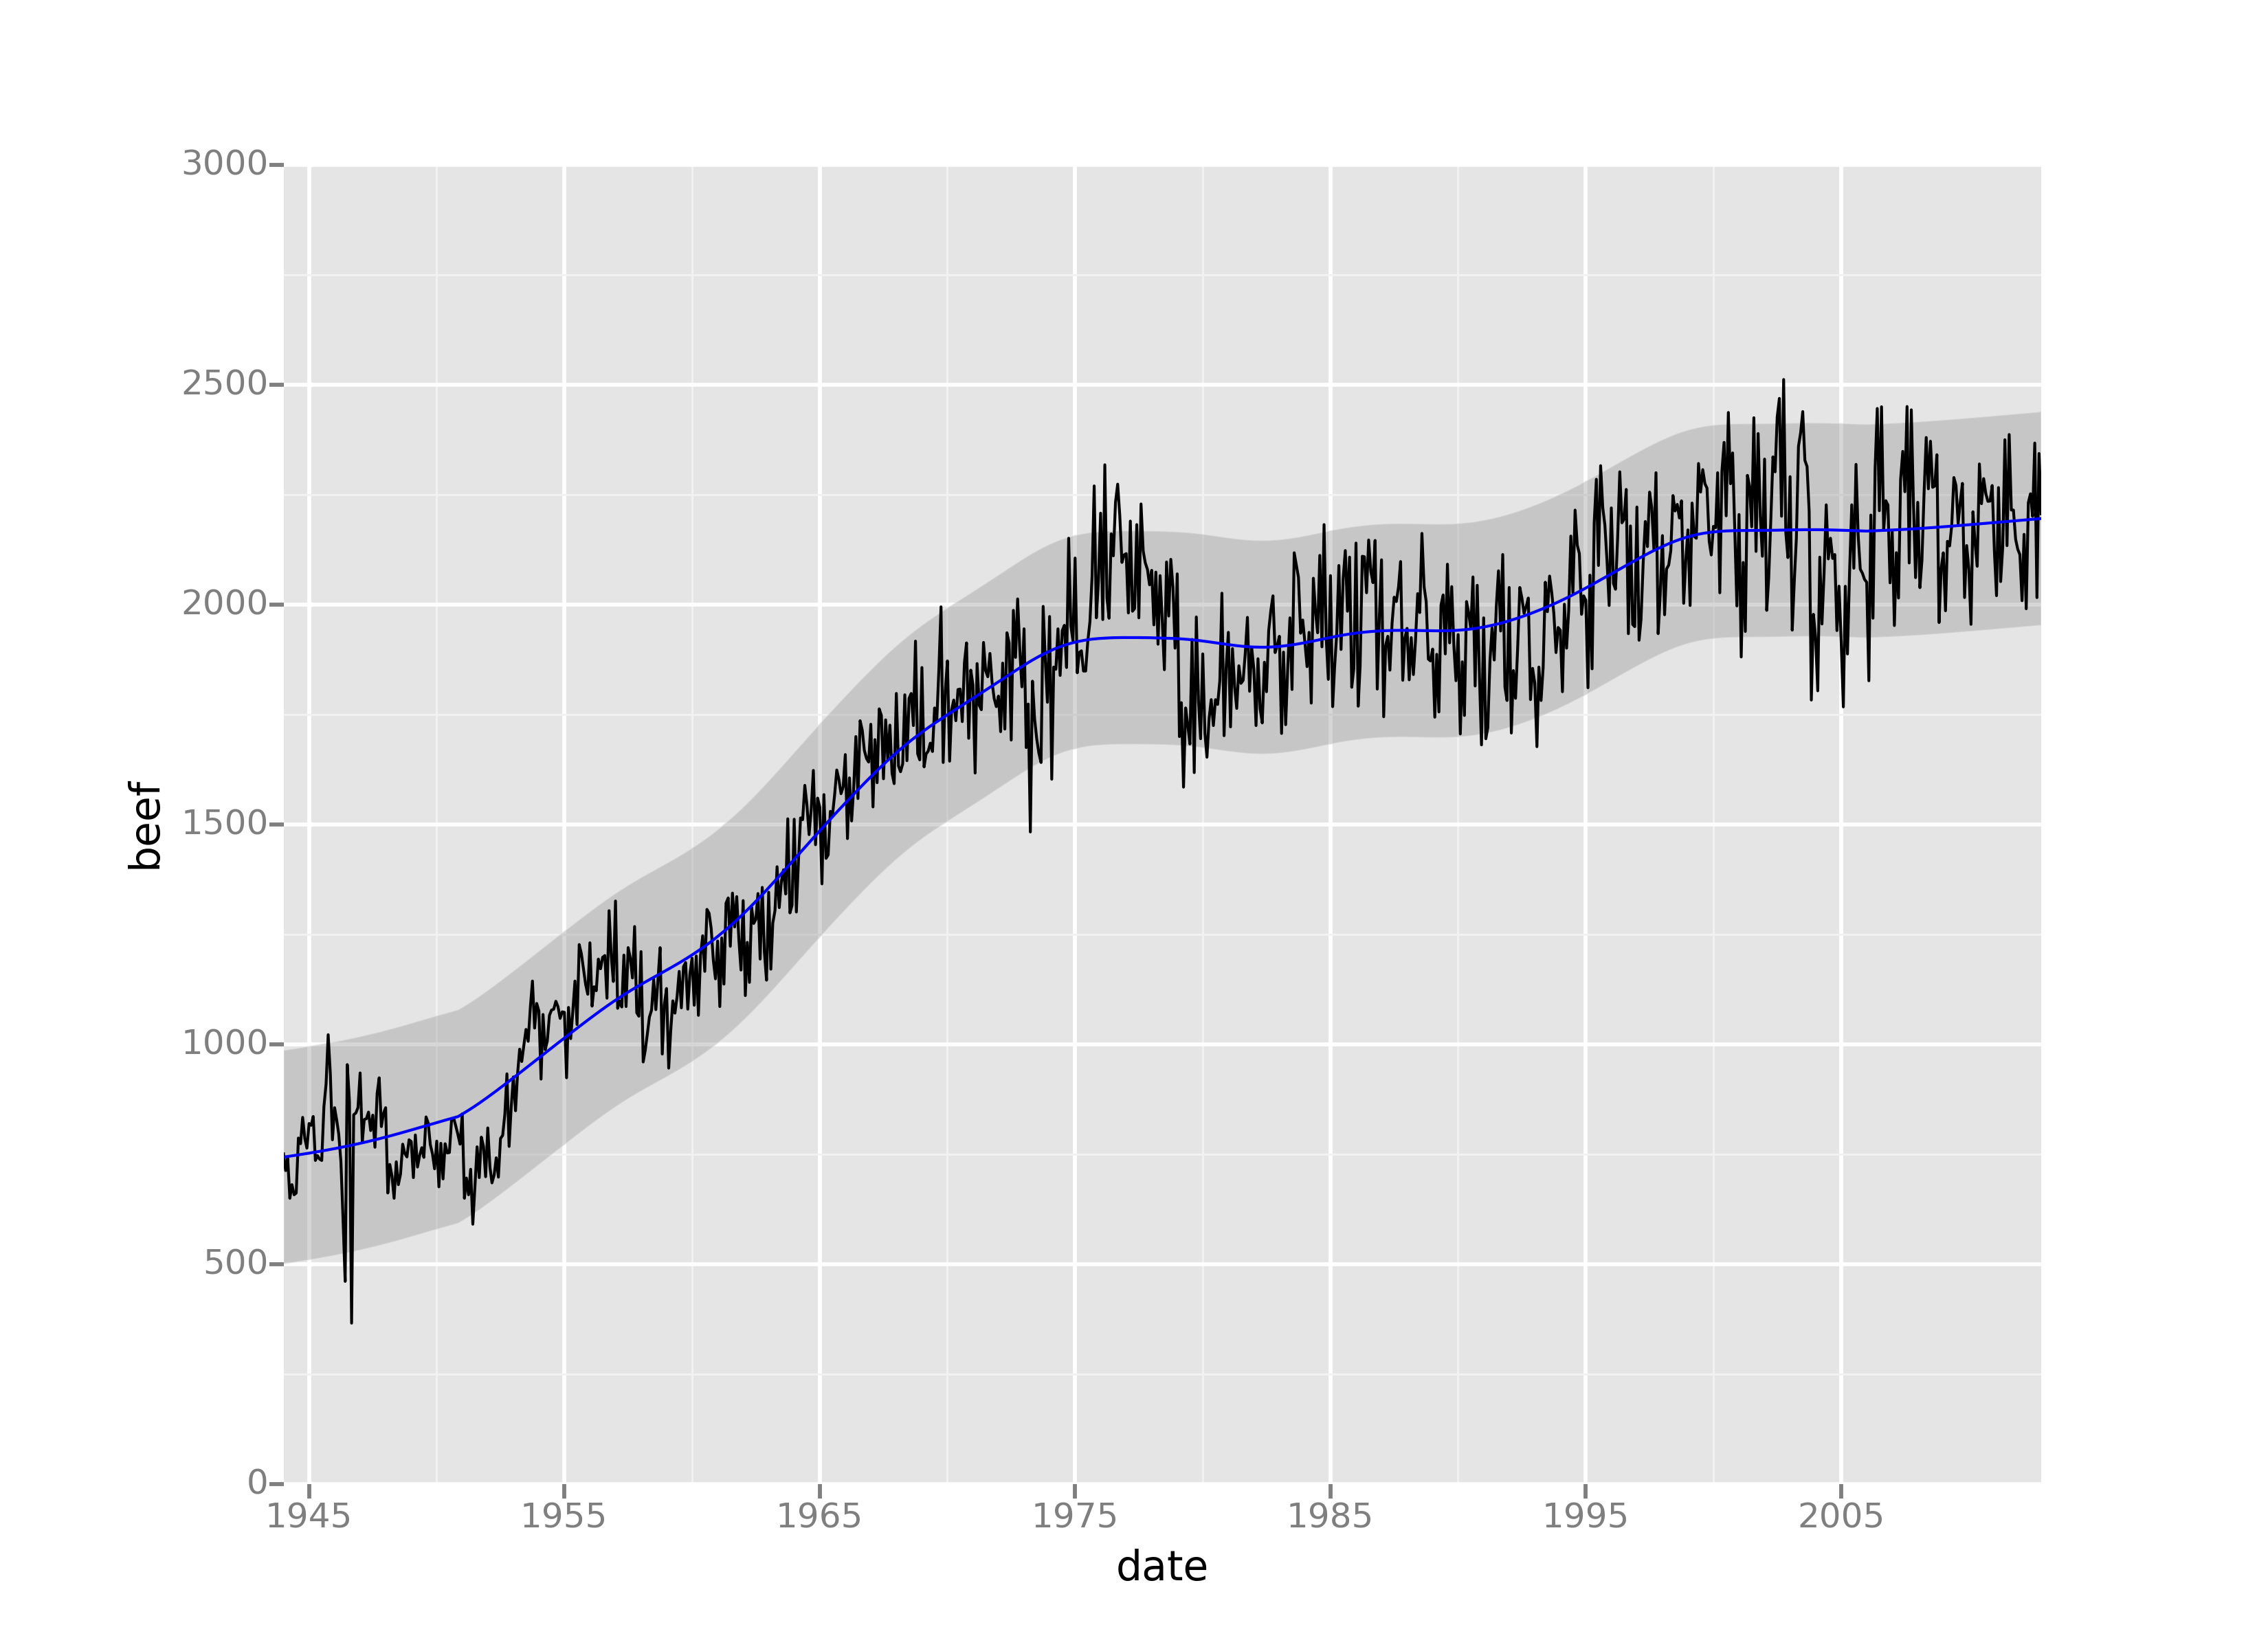
\includegraphics[width=1.1\linewidth]{stats1}
	\end{figure}
\end{frame}
%==================================== %
\begin{frame}
	\frametitle{stats for ggplot}
	\Large
	These are the stats currently available for ggplot in python.\\
	\bigskip
	\begin{center}
		\begin{tabular}{|c|c|}\hline
			stat\_abline	&	stat\_hline	\\ \hline
			stat\_bar	&	stat\_identity	\\ \hline
			stat\_bin	&	stat\_smooth	\\ \hline
			stat\_bin2d	&	stat\_summary	\\ \hline
			stat\_density	&	stat\_vline	\\ \hline
			stat\_function	&		\\ \hline
		\end{tabular} 
	\end{center}
\end{frame}
%================================================ %
%\begin{frame}[fragile]
%	\frametitle{Aesthetics}
%	\Large
%	\noindent \textbf{Aesthetics}
%	\begin{itemize}
%		\item Aesthetics describe how your data will relate to your plots.
%		\item Some common aesthetics are: \textbf{x}, \textbf{y}, and \textbf{color}. \item Aesthetics are specific to the type of plot (or layer) you're adding to your visual. 
%		\item For example, a scatterplot (\texttt{geom\_point}) and a line (\texttt{geom\_line}) will share x and y, but only a line chart has a linetype aesthetic.
%	\end{itemize}
%	
%	
%	%For more information about which geoms have which aesthetics, see the DOCS SECTION.
%\end{frame}
\section{qplot}

\begin{frame}
	\frametitle{qplot}
	\Large
	\noindent \textbf{quickplot}
	\begin{itemize}
		\item \texttt{qplot()} is the basic plotting function in the ggplot package, designed for quick inspections of the data.
		\item The functionality is not as expansive as with using ``\texttt{ggplot()}".
		\item For the most part, the same code works for both.
	\end{itemize}
	
\end{frame}
%================================================================================== %
%\begin{frame}[fragile]
%	\frametitle{Aesthetics}
%	\Large
%	Aesthetics correspond with the ``X" and ``Y" variables. The first line of the code below indicates which variable is which.
%	\begin{framed}
%		\begin{verbatim}
%		ggplot(aes(x=date,y=beef, meat2) +
%		geom_line() +
%		stat_smooth(colour="blue", span=0.2)
%		\end{verbatim}
%	\end{framed}
%	
%\end{frame}

\section{Faceting}


%========================================%
\begin{frame}[fragile]
	\frametitle{ggplot2 - faceting}
	\large
	\noindent \textbf{Facetting}
	\begin{itemize}
		\item One of the most useful techniques in data visualization is rendering groups of data alongside each other, making it easy to compare the groups.
		\item With ggplot2, one way to do this is by mapping a discrete variable to an aesthetic, like x position, color, or shape.
		\item Another way of doing this is to create a subplot for each group and draw the subplots side by side.
		\item ggplot2 has two ways to do this: \texttt{facet\_grid()} and \texttt{facet\_wrap()}.
	\end{itemize}
\end{frame}
\begin{frame}
	\Large
	\noindent \textbf{Faceting}\\
	The faceting approach supported by ggplot partitions a plot into a matrix of panels. Each panel shows a different subset of the data.
	There are two faceting approaches:
	
	\begin{itemize}
		\item \texttt{facet\_wrap("cell")} - univariate: create a 1-d strip of panels, based on one factor, and wrap the strip into a 2-d matrix
		\item \texttt{facet\_grid("row","col")} - (usually) bivariate: create a 2-d matrix of panels, based on two factors
	\end{itemize}
\end{frame}
%================================ %
\begin{frame}[fragile]
	\frametitle{Faceting}
\Large
\noindent \textbf{Quick Example of Faceting}\\
Suppose \texttt{cyl} and \texttt{drv} are two categorical variables in the \textbf{mpg} data frame
\begin{framed}
\begin{verbatim}
qplot(.....) + facet_grid(cyl,drv)
\end{verbatim}
\end{framed}

\end{frame}
%================================ %
\begin{frame}
	\frametitle{Faceting}
	\begin{figure}
\centering
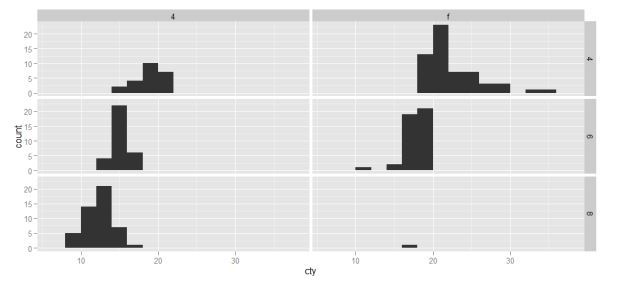
\includegraphics[width=1.1\linewidth]{gridfacetting}
\caption{Grid Faceting}
\label{fig:gridfacetting}
\end{figure}

\end{frame}


%================================ %
\begin{frame}
	\frametitle{Faceting}
\Large
\vspace{-1cm}
\noindent \textbf{Facet Wrap}
\begin{itemize}
\item An alternative to grid facetting is a wrapped ribbon of plots
\item \texttt{facet\_wrap} generates a long ribbon of plots, and wraps it into 2d.
\end{itemize}

\end{frame}




%========================================%
\begin{frame}[fragile]
\frametitle{ggplot2 - faceting}
	\large
\noindent \textbf{Facet Grid}\\
With \texttt{facet\_grid()}, you can specify a variable to split the data into vertical subpanels, and another variable to split it into horizontal subpanels
\begin{framed}
		\begin{verbatim}
		# The base plot
		p <- ggplot(diamonds, 
		 aes(x = price, y = depth)) + geom_point()
		
		# Faceted by color
		# vertically arranged subpanels
		p + facet_grid(color ~ .)
		\end{verbatim}
	\end{framed}
\end{frame}


%========================================%
\begin{frame}[fragile]
	\frametitle{ggplot2 - faceting}
	
	\begin{framed}
		\begin{verbatim}
		# Faceted by clarity
		# in horizontally arranged subpanels
		
		p + facet_grid(. ~ clarity)
		\end{verbatim}
	\end{framed}
\end{frame}
%========================================%
\begin{frame}[fragile]
	\frametitle{ggplot2 - faceting}
	
\noindent	\textbf{Putting Both Together}
	\begin{framed}
		\begin{verbatim}
		
		
		# Split by color (vertical) and clarity (horizontal)
		p + facet_grid(color ~ clarity)
		
		\end{verbatim}
	\end{framed}
\end{frame}
%========================================%
\begin{frame}[fragile]
	\frametitle{ggplot2 - faceting}

	\begin{figure}
\centering
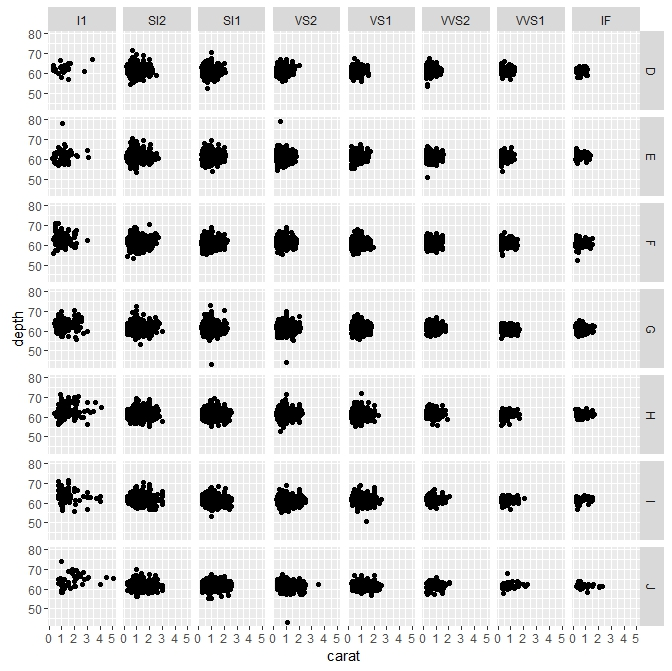
\includegraphics[width=0.7\linewidth]{diamondsfacetgrid}

\end{figure}

\end{frame}
%========================================%
\begin{frame}[fragile]
	\frametitle{ggplot2 - faceting}
	\large
\noindent \textbf{Facet Wraps}
\begin{itemize}
\item \texttt{facet\_wrap()} creates and labels a plot for every level of a factor which is passed to it.
\item The primary argument takes the form of a one sided formula: $\sim$\texttt{Factor}.
\item this will then efficiently ``wrap” these plots into a 2d grid.
\end{itemize}
\begin{framed}
\begin{verbatim}
p + facet_wrap(~clarity)
\end{verbatim}
\end{framed}
\end{frame}
%========================================%
\begin{frame}[fragile]
\frametitle{ggplot2 - faceting}
\begin{framed}
\begin{verbatim}
# These will have the same result: 
# 2 rows and 4 cols

p + facet_wrap(~clarity, nrow = 2)

p + facet_wrap(~class, ncol = 4)

#Try some variants of this 
\end{verbatim}
\end{framed}
\end{frame}
%========================================%
\begin{frame}[fragile]
	\frametitle{ggplot2 - faceting}
	\large
\noindent \textbf{Facet Scales}
	\begin{itemize}
\item	Usually you will want all of your facets to have the same x and y scales.
\item  If you're plotting the same data in each facet, having free scales on each of the facets will ruin comparability across facets.
\item However, sometimes it will be appropriate to have free scales. You can do this by passing \texttt{scales = "free"} to \texttt{facet\_wrap()}.
	\end{itemize}

	\begin{framed}
		\begin{verbatim}
		p + facet_wrap(~clarity, scales = "free")
		\end{verbatim}
	\end{framed}
\end{frame}
%========================================%


%============================================= %


\begin{frame}
	\begin{figure}
		\centering
		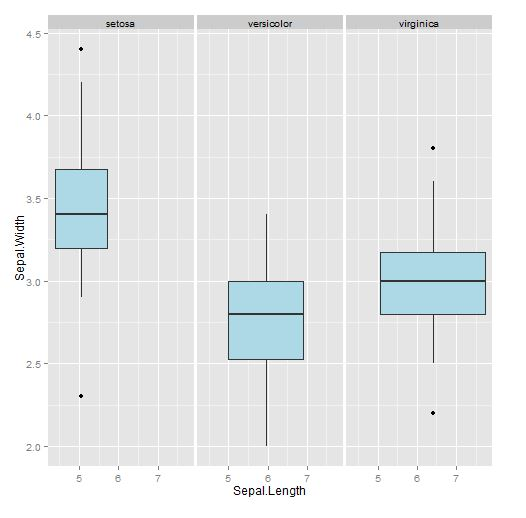
\includegraphics[width=0.7\linewidth]{iris-boxplot}
	\end{figure}
	
\end{frame}

%================================= %
\section*{Scales}
% http://sape.inf.usi.ch/quick-reference/ggplot2/scale
\begin{frame}
	\Large
	\vspace{-0.7cm}
\noindent \textbf{Scales and Themes}
	\begin{itemize}
	\item ggplot2 provides a large number of scale functions
	to control aspects of a graphic including axes and
	legends
	\item theme functions allow us to control the overall style
	of the graphic
	\end{itemize}

\end{frame}

\begin{frame}
	\Large
		\vspace{-0.7cm}
	\noindent \textbf{Scales}
	\begin{itemize}
		\item A scale determines how an attribute of the data is mapped into an aesthetic property of a \texttt{geom} (e.g., the geom's position along the x axis, or a geom's fill color in a color space).
		\item The colours and shapes used in the chart can be manually adjusted if you don’t like the defaults.
	\end{itemize}
	
\end{frame}
%================================== %
\section{Themes}
\begin{frame}[fragile]
\frametitle{Themes}
\Large
	\begin{framed}
	\begin{verbatim}
	ggplot(aes(x=date, y=beef), meat2) +
			geom_line() +
			theme_bw()
	\end{verbatim}
	\end{framed}
\end{frame}
%============================ %
\begin{frame}
\frametitle{Themes}
\Large
\begin{figure}
\centering
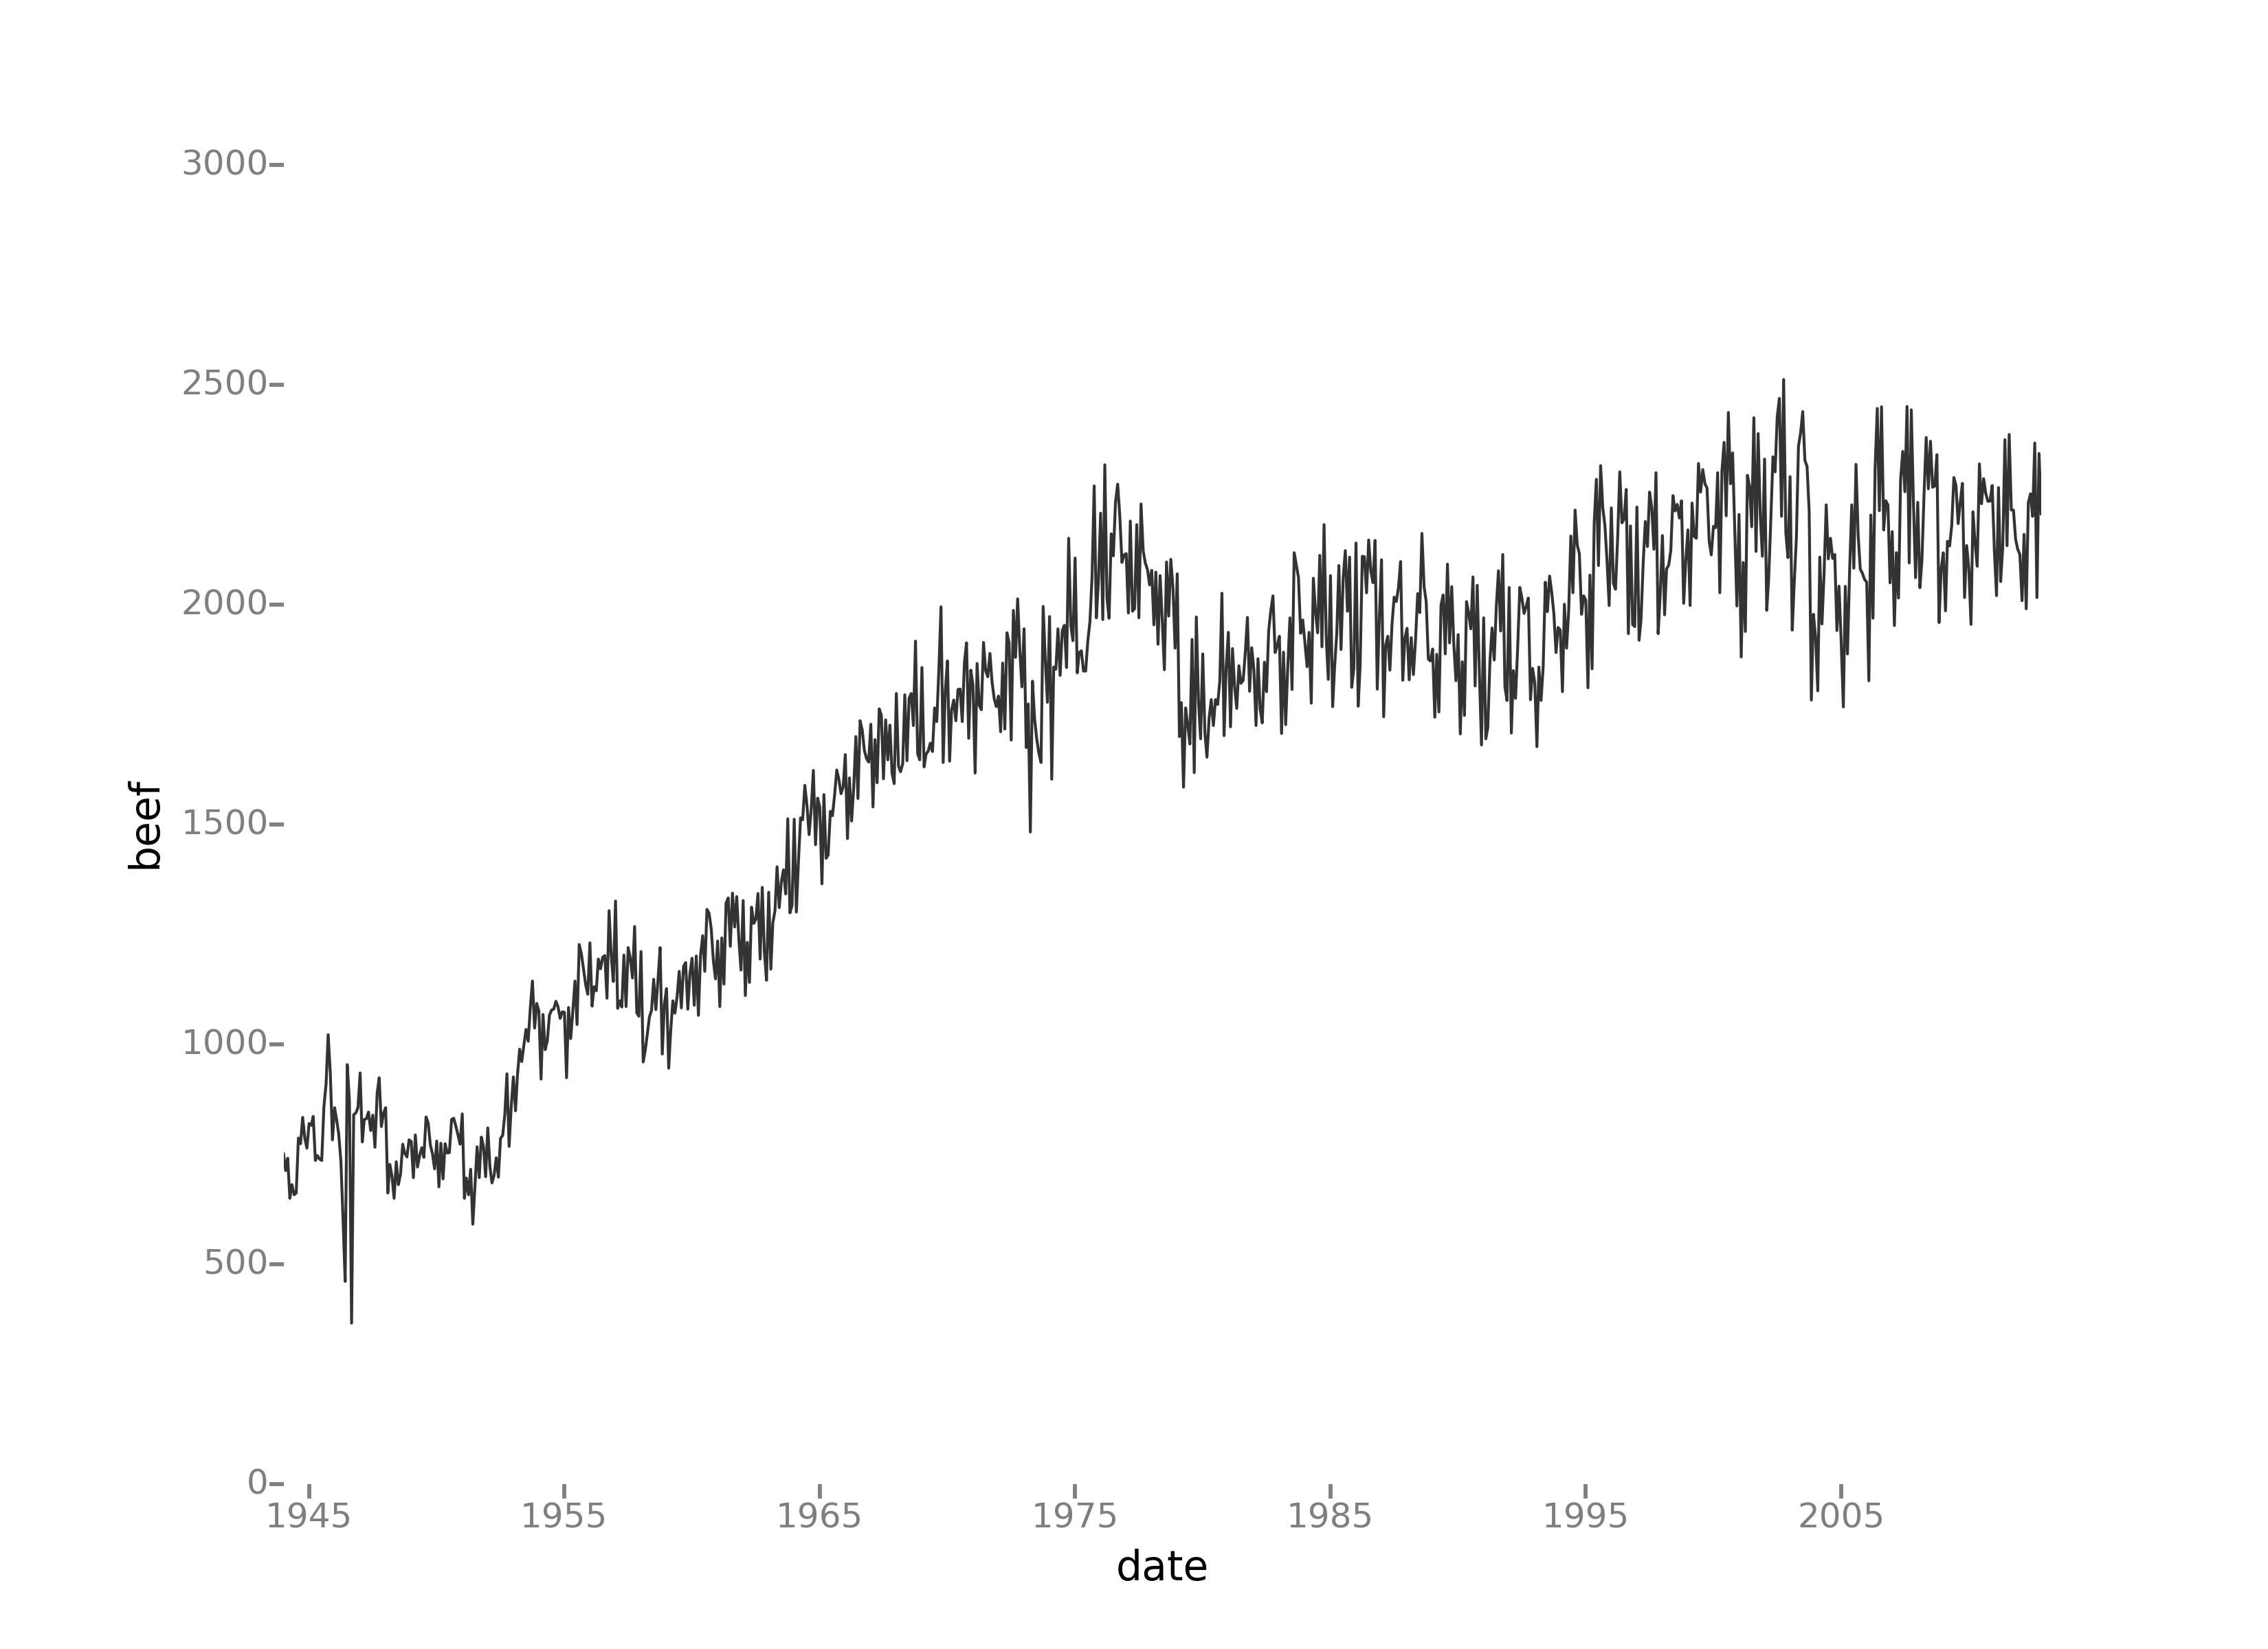
\includegraphics[width=1.0\linewidth]{meat_theme_bw}
\end{figure}

\end{frame}
%===========================================%
\begin{frame}
\frametitle{Themes}
\Large
Try out the following themes: 
\smallskip
	\begin{itemize}
		\item	\texttt{theme\_538}
		\item	\texttt{theme\_bw}
		\item	\texttt{theme\_gray}
		\item	\texttt{theme\_matplotlib}
		\item	\texttt{theme\_seaborn}
		\item	\texttt{theme\_xkcd}
	\end{itemize}
	
\end{frame}
\end{document}
